\documentclass{beamer}

\usetheme{Boadilla}

%\includeonlyframes{current}

\usepackage{times}
\usefonttheme{structurebold}
\usepackage{listings}
\usepackage{ragged2e}

\usepackage{pgf}
\usepackage{tikz}
\usepackage{alltt}
\usepackage[normalem]{ulem}
\usetikzlibrary{arrows}
\usetikzlibrary{automata}
\usetikzlibrary{shapes}
\usepackage{amsmath,amssymb}
\usepackage{rotating}
\usepackage{ulem}
\usepackage{listings}
\usepackage{enumerate}
\usepackage{tikz}
\tikzset{
  every overlay node/.style={
    draw=black,fill=white,rounded corners,anchor=north west,
  },
}
\def\tikzoverlay{%
   \tikz[baseline,overlay]\node[every overlay node]
}%

%\setbeamercovered{dynamic}
\setbeamertemplate{footline}[page number]{}
\setbeamertemplate{navigation symbols}{}
\usefonttheme{structurebold}

\title{Software Testing, Quality Assurance \& Maintenance---Lecture 21}
\author{Patrick Lam}
\date{February 27, 2015}

\colorlet{redshaded}{red!25!bg}
\colorlet{shaded}{black!25!bg}
\colorlet{shadedshaded}{black!10!bg}
\colorlet{blackshaded}{black!40!bg}

\colorlet{darkred}{red!80!black}
\colorlet{darkblue}{blue!80!black}
\colorlet{darkgreen}{green!80!black}

\newcommand{\rot}[1]{\rotatebox{90}{\mbox{#1}}}
\newcommand{\gray}[1]{\mbox{#1}}

\newenvironment{changemargin}[1]{% 
  \begin{list}{}{% 
    \setlength{\topsep}{0pt}% 
    \setlength{\leftmargin}{#1}% 
    \setlength{\rightmargin}{1em}
    \setlength{\listparindent}{\parindent}% 
    \setlength{\itemindent}{\parindent}% 
    \setlength{\parsep}{\parskip}% 
  }% 
  \item[]}{\end{list}}


\lstset{ %
language=C++,
basicstyle=\ttfamily,commentstyle=\scriptsize\itshape,showstringspaces=false,breaklines=true}

\begin{document}

\begin{frame}
  \titlepage
\end{frame}

\begin{frame}
\frametitle{Today}
\begin{changemargin}{2cm}
Midterm Review!
\end{changemargin}
\end{frame}

\begin{frame}
  \frametitle{Coverage}

\large
  \begin{changemargin}{2em}
Idea: find a reduced space and cover it with tests.\\[1em]

Seen so far: graph (structural, dataflow); syntax.
  \end{changemargin}
  
\end{frame}

\begin{frame}
  \frametitle{How Code Goes Bad}
  \begin{changemargin}{1cm}
\begin{itemize}
\item {\bf Fault} (also known as a bug): A static defect in software---incorrect lines of code.
\item {\bf Error}: An incorrect internal state---follows execution of a fault, but not necessarily observed yet.
\item {\bf Failure}: External, incorrect behaviour with respect to the expected behaviour---must be visible (e.g. EPIC FAIL).
\end{itemize}

\begin{center} --- and  --- 
\end{center}

to manifest a failure (RIP):
\begin{enumerate}
\item Fault must be {\bf reachable};
\item Program state subsequent to reaching fault must be incorrect: {\bf infection}; and
\item Infected state must {\bf propagate} to output to cause a visible failure.
\end{enumerate}
  \end{changemargin}
  
\end{frame}

\begin{frame}
  \frametitle{Talking about Coverage Criteria}

  \begin{changemargin}{1cm}
  Let's go top-down.\\[1em]

  {\bf Coverage criterion:} \\
  \hspace*{2cm} imposes a set of {\bf test requirements} (TRs);\\
  \hspace*{2cm} a {\bf test set} may cover a set of TRs.\\[1em]

  {\bf Test requirement:} \\
  \hspace*{2cm} a condition that some {\bf test case} must satisfy.\\[1em]

  {\bf Test set:} \\
  \hspace*{2cm} a collection of {\bf test cases}.\\[1em]
  
  {\bf Test case:} \\
  \hspace*{2cm} a set of inputs \& corresponding expected outputs\\
  \hspace*{3cm} (+prefix values, +postfix values).\\
  
  \end{changemargin}
  
\end{frame}

\begin{frame}
  \frametitle{Subsumption}

  \begin{changemargin}{2cm}
    Sometimes, any test set that satisfies criterion X \\ will also satisfy criterion Y.\\[1em]
    Then we say that X {\bf subsumes} Y.\\[1em]
    This is a mostly-theoretical point; \\
    in particular, some criteria are hard to use,\\
    and it's always impractical to get to 100\% anyway.\\[1em]
    There is a subsumption chart in the notes. \\
    Look at it.
  \end{changemargin}
\end{frame}

\part{Graph Coverage}
\begin{frame}
\partpage
\end{frame}

\begin{frame}
  \frametitle{Terms for Graphs}

  \begin{changemargin}{2cm}
    \begin{itemize}
    \item path, subpath, subsequence;
    \item test path;
      \begin{itemize}
    \item test path(s) induced by a test case (path$_G$(t))
    \item nondeterminism and test paths;
      \end{itemize}
    \item reachability: semantic and syntactic.
    \end{itemize}
    ~\\[1em]
    Note: sets of test paths satisfy coverage criteria,\\ \hspace*{2cm} but we run test cases.
  \end{changemargin}
\end{frame}

\begin{frame}
  \frametitle{Criteria You'll Encounter Later}

  \Large
  \begin{changemargin}{2cm}
    \begin{itemize}
    \item Node Coverage (NC). \\ \hspace*{2em} (aka statement coverage)
    \item Edge Coverage (EC). \\ \hspace*{2em} (aka branch coverage)
    \end{itemize}
  \end{changemargin}
\end{frame}

\begin{frame}
  \frametitle{No one but us cares about these graph criteria}

  \Large
  \begin{changemargin}{1cm}
    \begin{itemize}
    \item Edge Pair Coverage (EPC)
    \item Prime Path Coverage (PPC)
    \item Complete Path Coverage (CPC)
    \item Prime Path Coverage (PPC)
    \item Simple/Complete Round Trip Coverage \\ \hspace*{2cm} (SRTC/CRTC)
    \item Specified Path Coverage (SPC)
      \item Bridge Coverage (BC)
    \end{itemize}
~\\[1em]
    (\ldots but they are fair game for exams.)
  \end{changemargin}
\end{frame}


\begin{frame}
  \frametitle{Graphs and Code}
  \begin{changemargin}{2cm}
    Be able to draw Control Flow Graphs.\\
    \hspace*{1cm} (\& basic blocks)
  \end{changemargin}
\end{frame}

\begin{frame}
  \frametitle{Data flow criteria}
  \begin{changemargin}{2cm}
    Seem like a good idea: \\
    \hspace*{1cm} focus on movement of data around a program.\\[1em]
    Terms:
    \begin{itemize}
    \item def, use, du-pair;
    \item def \emph{reaches} a use along a \emph{def-clear} path;
    \item du-path;
    \item def-path set, def-pair set;
      \item All-Defs Coverage, All-Uses Coverage.
    \end{itemize}
  \end{changemargin}
\end{frame}

\begin{frame}
  \frametitle{Data flow criteria and Call Graphs}
  \begin{changemargin}{2cm}
    nodes: methods; edges: method calls.\\[1em]
    last-def/first-use optimization
  \end{changemargin}
\end{frame}

\begin{frame}
  \frametitle{Graph Coverage Criteria in Practice}
  \begin{changemargin}{1cm}
    Industry uses statement coverage and branch coverage.\\
      \hspace*{2em} (easy to measure)\\[1em]
      But, what do they mean?
      \begin{enumerate}
      \item Low coverage: your code is untested!
      \item High coverage: \ldots well, who knows?
      \end{enumerate}~\\[.5em]
      Research shows that bigger suites detect more bugs,\\
      and higher-coverage suites are bigger,\\
      but not that higher coverage is intrinsically better.
  \end{changemargin}
\end{frame}
      
\part{Syntax-Based Testing}
\begin{frame}
\partpage
\end{frame}

\begin{frame}
  \frametitle{Two Ways of using Grammars}
  \begin{changemargin}{2cm}
    \Large
    \begin{itemize}
    \item input spaces
    \item programs (mutation testing)
    \end{itemize}
  \end{changemargin}
\end{frame}

\begin{frame}
  \frametitle{Input Spaces}
  \begin{changemargin}{1.5cm}
    \Large
    Test case generation:
    \begin{itemize}
    \item generate valid inputs from grammar;
    \item generate invalid inputs by modifying grammar.
    \end{itemize}~\\
    Can use grammar mutation operators to modify grammar.
  \end{changemargin}
\end{frame}

\begin{frame}
  \begin{center}
  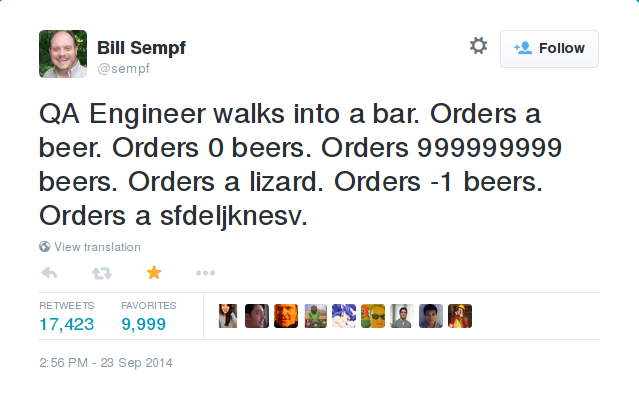
\includegraphics[width=.8\textwidth]{L21/sempf-tweet}
\hfill  \url{https://twitter.com/sempf/status/514473420277694465}
  \end{center}
\end{frame}

\begin{frame}
    \frametitle{Mutation Testing}
  \begin{center}
    
\includegraphics[width=.6\textwidth]{L21/Xav-lopr}
    \hfill \url{http://en.wikipedia.org/wiki/File:Xav-lopr.png}
  \end{center}
\end{frame}

\begin{frame}
  \frametitle{Mutation Testing: Key Idea}
  \begin{changemargin}{2cm}
    \Large
    Improve test suites\\ by forcing them to detect \\ known-wrong programs.
  \end{changemargin}
\end{frame}

\begin{frame}
  \frametitle{Carrying out Mutation Testing}
  \begin{changemargin}{2cm}
    \Large
    \begin{enumerate}
    \item generate mutants;
    \item eliminate equivalent mutants;
    \item ensure tests {\bf kill} enough mutants \\
      (add tests if necessary).
    \end{enumerate}
  \end{changemargin}
\end{frame}

\begin{frame}
  \frametitle{Why Mutation Testing is Hard}
  \begin{changemargin}{2cm}
    \Large
    Tools can generate mutants for you.\\[1em]
    But you must still:
    \begin{enumerate}
  \item figure out equivalence;
  \item design a test case \\
    \hspace*{2em} to kill the mutant.
    \end{enumerate}
  \end{changemargin}
\end{frame}

\begin{frame}
  \frametitle{Is mutation testing all worth it?}

  \begin{changemargin}{2cm}
    \Large
    Yes, probably.\\[1em]
    Test suites which kill mutants\\
    also detect real bugs.
  \end{changemargin}
\end{frame}

\part{Concurrency Bugs}
\begin{frame}
\partpage
\end{frame}

\begin{frame}
  \frametitle{Problems with concurrency}

  \begin{changemargin}{2cm}
    \Large
    \begin{itemize}
  \item race conditions;
  \item atomicity violations;
  \item deadlocks.
    \end{itemize}
  \end{changemargin}
\end{frame}

\begin{frame}[fragile]
  \frametitle{Detecting lock problems: paired calls}
    \begin{lstlisting}[language=C,commentstyle={\color{red}\bf}]
/* 2.4.0:drivers/sound/cmpci.c:cm_midi_release: */
lock_kernel(); // [PL: GRAB THE LOCK]
if (file->f_mode & FMODE_WRITE) {
  add_wait_queue(&s->midi.owait, &wait);
  ...
  if (file->f_flags & O_NONBLOCK) {
    remove_wait_queue(&s->midi.owait, &wait);
    set_current_state(TASK_RUNNING);
    return -EBUSY; // [PL: OH NOES!!1]
  }
  ...
}
unlock_kernel();
    \end{lstlisting}
    \begin{changemargin}{1cm}
      \Large
      Problem: lock() and unlock() must be paired!
  \end{changemargin}
\end{frame}

\begin{frame}[fragile]
\frametitle{aComment: inferring lock disciplines}
\begin{changemargin}{2cm}
  \begin{itemize}
  \item extract locking-related annotations from code;
  \item extract locking-related annotations from comments;
  \item propagate annotations to callers.
  \end{itemize}
\end{changemargin}
\end{frame}

\begin{frame}
\frametitle{Beliefs}
  \begin{changemargin}{2cm}
    MUST beliefs:\\
\hspace*{2em} violations are clearly wrong.\\[1em]
    MAY beliefs:\\
    \begin{itemize}
      \item need more evidence of wrongdoing.
    \end{itemize}
  \end{changemargin}
\end{frame}

\begin{frame}
\frametitle{General statistical technique}
  \begin{changemargin}{2cm}
``a(); \ldots b();'' implies MAY-belief that a() followed by b().\\
(is it real or fantasy? we don't know!)\\[2em]
Algorithm: 
\begin{itemize}
\item assume every {\tt a}--{\tt b} is a valid pair;
\item emit ``check'' for each path with ``a()'' and then ``b()'';
\item emit ``error'' for each path with ``a()'' and no ``b()''.
\end{itemize}
(actually, prefilter functions that look paired).
  \end{changemargin}
\end{frame}


\part{Tool Support}
\begin{frame}
\partpage
\end{frame}

\begin{frame}
  \frametitle{Laundry List I}
  \begin{changemargin}{2cm}
    \begin{itemize}
    \item iComment/aComment
    \item FindBugs
    \item Java Path Finder
    \item Korat
    \item Randoop
    \item Daikon
    \item ESC/Java
    \item Valgrind
    \item Flawfinder
    \end{itemize}
  \end{changemargin}
\end{frame}

\begin{frame}
  \frametitle{Laundry List II}
  \begin{changemargin}{2cm}
    \begin{itemize}
    \item Clang static analyzer
    \item cppcheck, sparse, splint
    \item pex
    \item KLEE
    \item Coverity, CodeSonar, Visual Studio
    \item PCLint, PVS-Studio, Fortify
    \item Intel Parallel Studio XE
    \item KlocWork Insight
    \item ScalaTest, ScalaCheck, Jacoco
    \item Atlassian Bamboo
    \end{itemize}
  \end{changemargin}
\end{frame}


% other tools (L12)
% must-beliefs, may-beliefs (L14)

\end{document}
